\documentclass[11pt,a4paper]{ctexart}
\usepackage[margin=2.2cm]{geometry}
\usepackage{amsmath,booktabs,graphicx,float,hyperref}
\hypersetup{colorlinks=true,urlcolor=blue}
\title{双层镍酸盐 RKKY 相互作用与 Sunny 基态计算}
\author{数值计算记录}
\date{2026年6月13日}
\begin{document}
\maketitle

\section{模型与参数}
紧束缚基底为 $(x_1,z_1,x_2,z_2)$。仅 $x^2-y^2$ 轨道作为巡游电子，
$z^2$ 轨道作为局域自旋。计算采用
$N_k=N_q=100$、$n=1.5$、$T=0.01$ eV、$J_K=1$ eV 和
$U=0:0.1:6$ eV。交换定义为
$J=-J_K^2\chi$，正 $J$ 对应反铁磁耦合。

Sunny 原胞包含面内坐标相同的上下两个格点，分数坐标为
$(0,0,0.25)$ 和 $(0,0,0.75)$。初始磁性超胞为
$4\times4\times1$，共 32 个自旋，$S=1/2$、$g=2$。
公共输入输出统一使用 eV；Sunny 0.8.0 内部数值临时转换为 meV。

\section{RKKY 结果}
正式扫描完成全部 61 个 $U$ 点。最大填充误差为
$9.9\times10^{-11}$，最大层对称残差为 $9.9\times10^{-15}$，
最大傅里叶虚部残差为 $1.4\times10^{-15}$。

\begin{figure}[H]
\centering
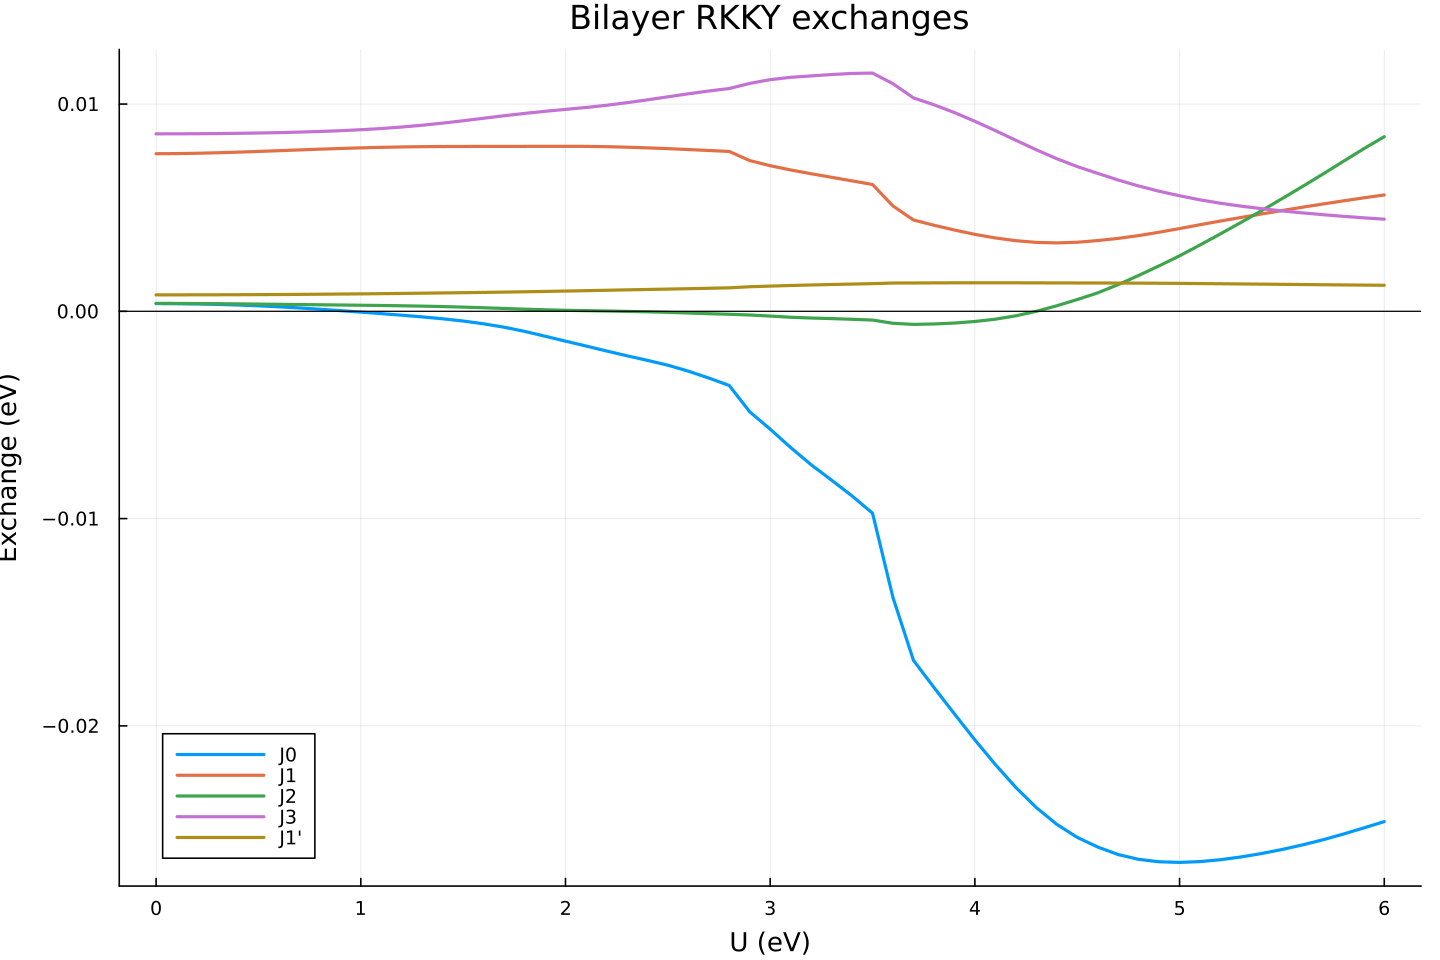
\includegraphics[width=0.92\textwidth]{../results/summary/rkky_exchanges.png}
\caption{五种交换常数随 $U$ 的变化。}
\end{figure}

\begin{table}[H]
\centering
\begin{tabular}{ccc}
\toprule
$U$ (eV) & $\max|J_{80}-J_{100}|$ (eV) & 是否补算 $N_k=120$\\
\midrule
0.0 & 1.494e-04 & yes \\
2.9 & 4.636e-05 & yes \\
3.0 & 4.185e-05 & no \\
3.6 & 3.270e-05 & yes \\
6.0 & 9.364e-05 & no \\
\bottomrule
\end{tabular}
\caption{动量网格收敛检查。小交换常数的相对误差会被放大，因此同时采用
$10^{-6}$ eV 的绝对阈值。}
\end{table}

\begin{figure}[H]
\centering
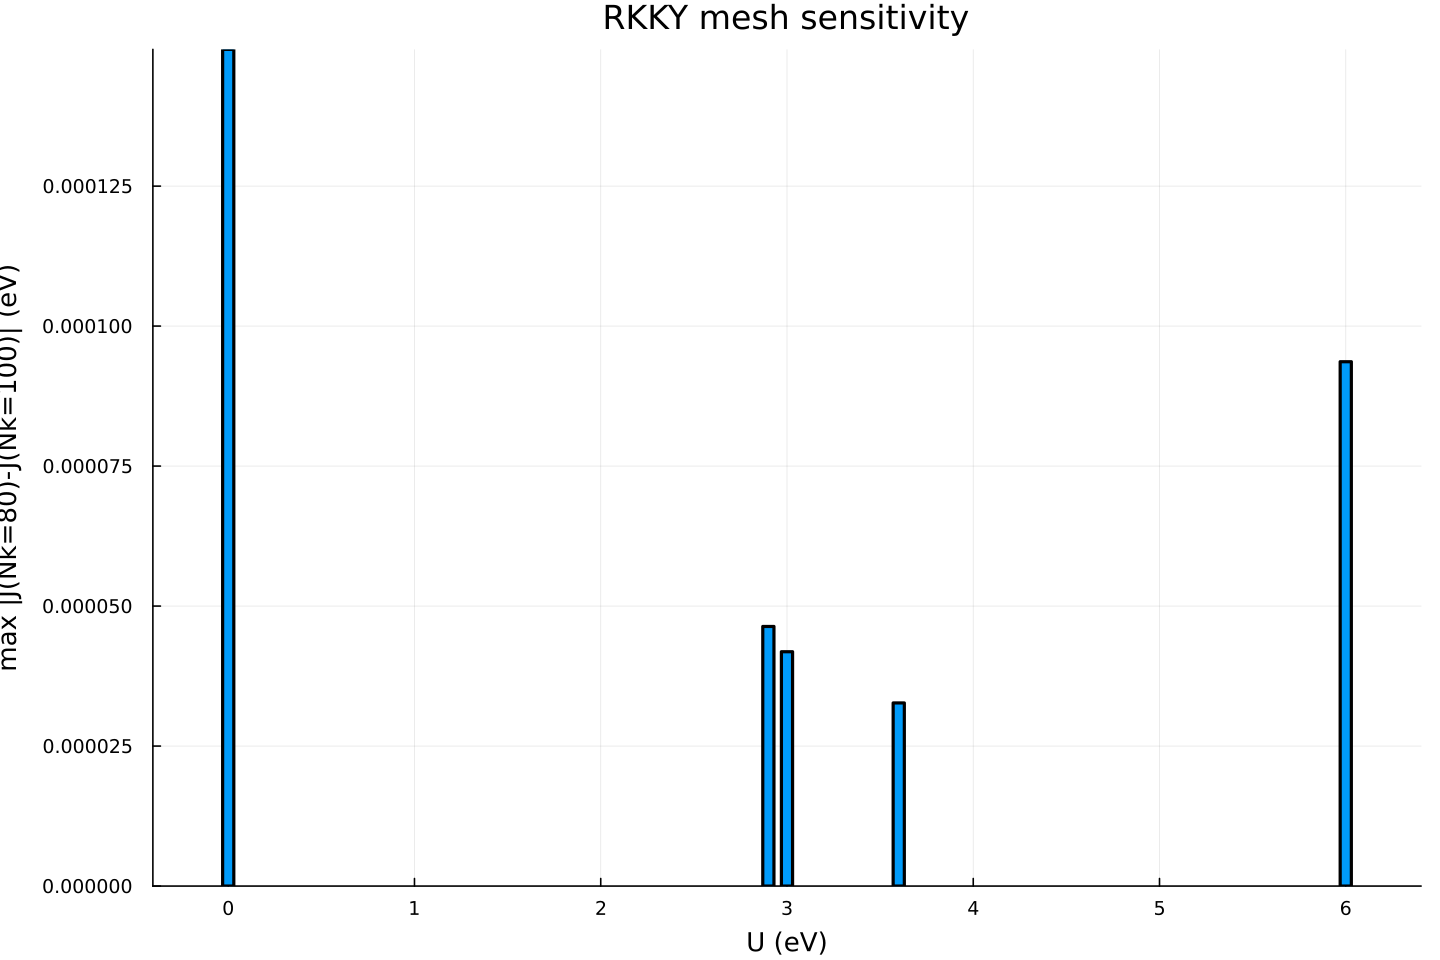
\includegraphics[width=0.78\textwidth]{../results/summary/rkky_convergence.png}
\caption{$N_k=80$ 与 100 的最大绝对差异。}
\end{figure}

\section{Sunny 基态相图}
有限超胞最小化在全部 $U$ 点均得到 period-4 家族的面内主峰。
$U\le0.9$ eV 时上下层反平行，$U\ge1.0$ eV 时上下层平行；
因此离散扫描只能将层间相变定位在 $0.9<U<1.0$ eV。
61 个选中结果中有 56 个未触发最小化器收敛警告。

\begin{figure}[H]
\centering
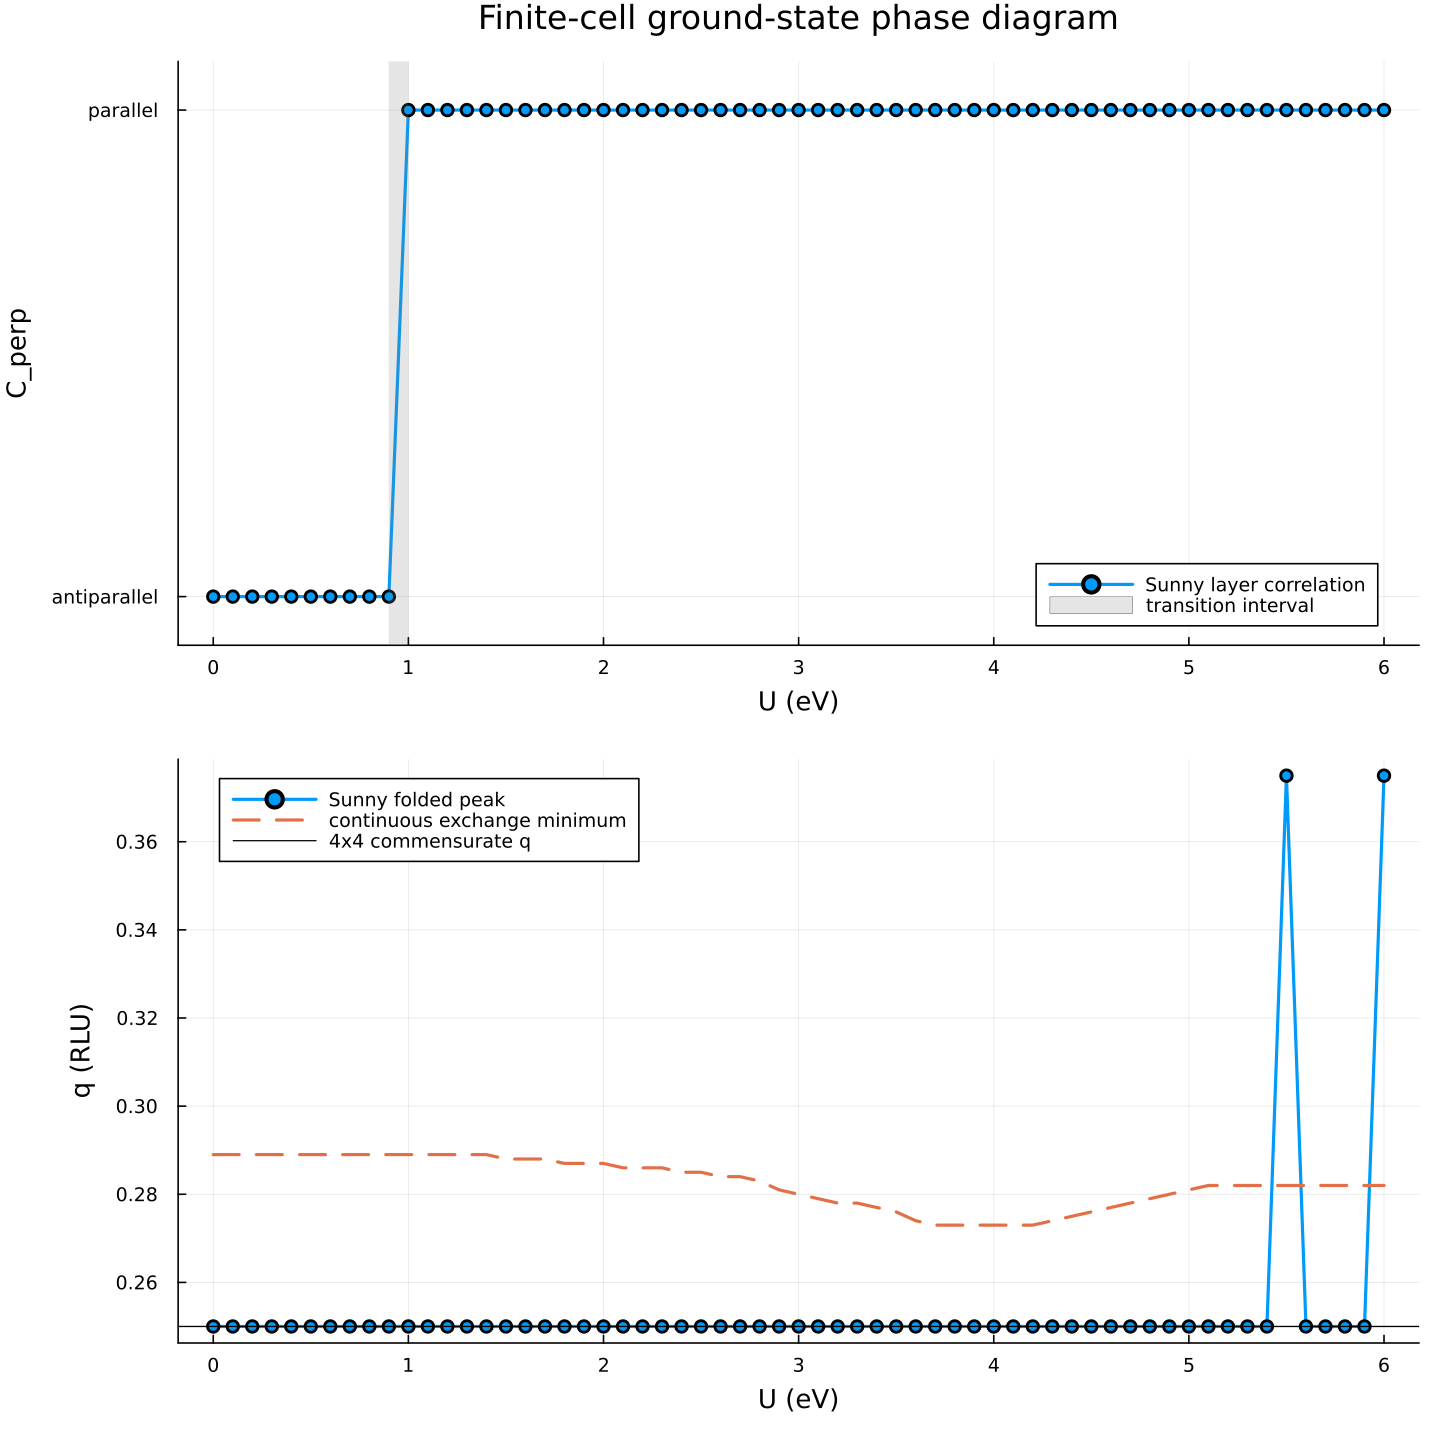
\includegraphics[width=0.90\textwidth]{../results/summary/ground_state_phase_diagram.png}
\caption{上：层间关联给出的有限胞相图。下：Sunny 有限胞结构因子主峰与
连续交换矩阵最低波矢的比较。}
\end{figure}

\begin{figure}[H]
\centering
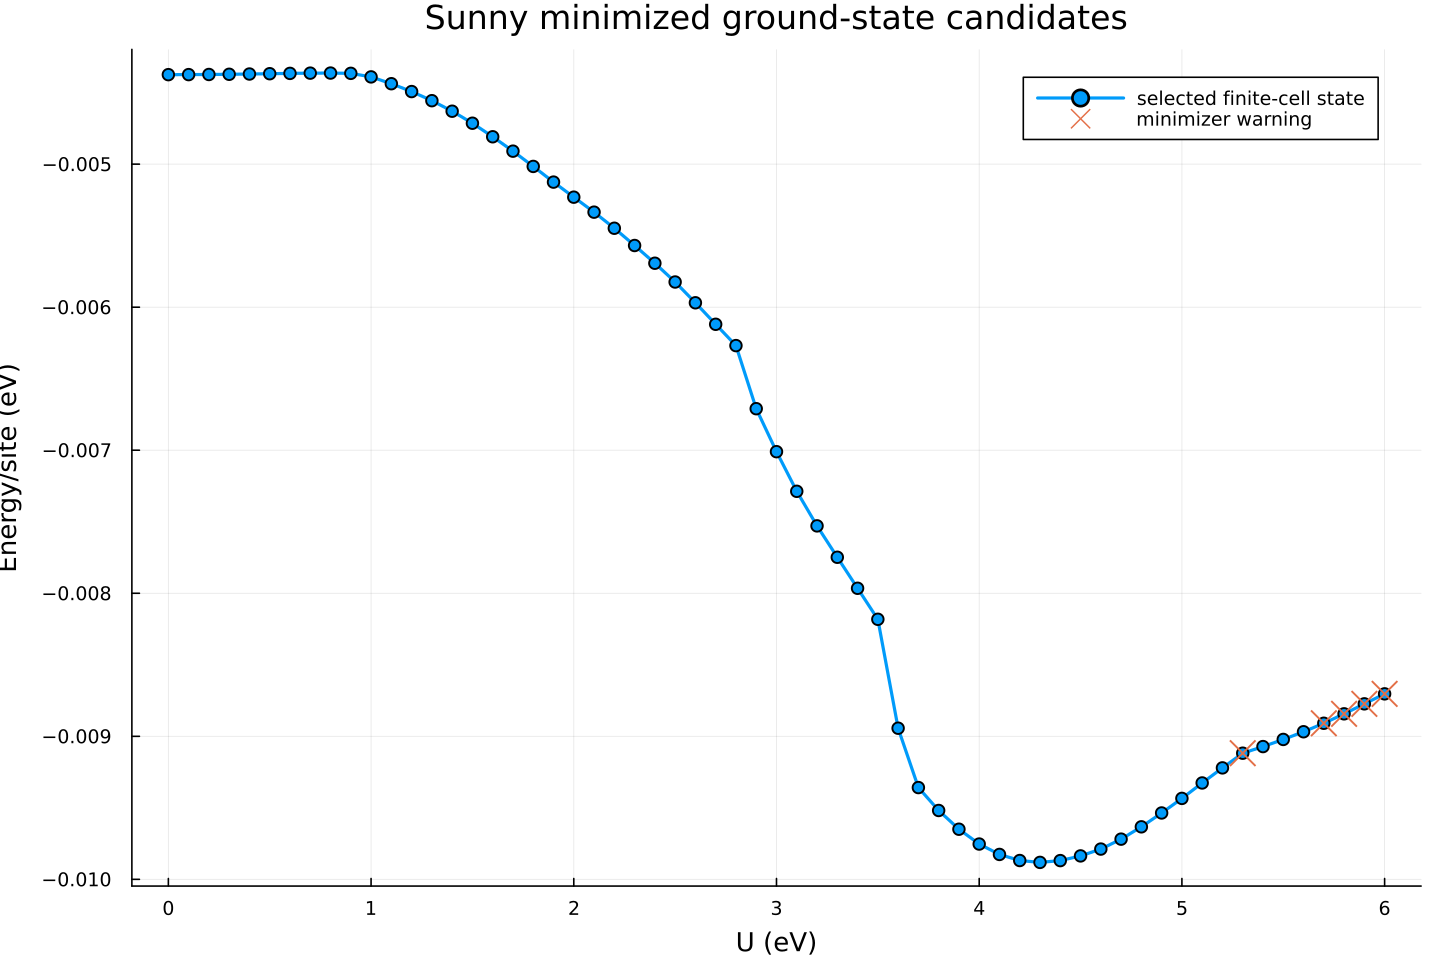
\includegraphics[width=0.78\textwidth]{../results/summary/ground_state_energy.png}
\caption{每个 $U$ 选中尝试的基态候选能量。叉号表示最小化器给出收敛警告。}
\end{figure}

\section{自旋波失稳}
Sunny 在 61/61 个参数点均抛出自旋波失稳异常，因此没有把
无效结果伪装成正常色散图。每点均执行了最多九次协议：4x4 五个种子、
6x6 两个种子和 8x8 两个种子，并保存异常消息、失稳波矢、基态和全部尝试。
对应诊断图保存在 \texttt{results/excitations}。

连续交换矩阵的最低点约在 $(0.273,0.273)$--$(0.289,0.289)$ RLU，
而 4x4 超胞只能表示四分之一间隔的波矢。该不公度最低点与有限超胞
period-4 近似之间的失配，会使有限胞构型不是无限晶格的严格局域极小值，
从而在磁性布里渊区的 $\Gamma$ 点附近产生负曲率。高 $U$ 端的 8x8
结果也出现偏离严格四分之一的主峰，支持这一解释。

部分重试同时给出最小化器未收敛警告，这会进一步增加失稳风险；但大量
已收敛尝试仍在相同近 $\Gamma$ 波矢失稳，说明问题不能仅归因于随机种子
或迭代次数。

\section{结论}
RKKY 交换常数已经可靠计算并通过网格检查。有限胞基态相图由两个主要区域
组成：低 $U$ 的 period-4/层间反平行态和高 $U$ 的
period-4/层间平行态。当前固定超胞下所有线性自旋波计算均失稳。
若后续需要物理色散，应改用 Sunny 的螺旋态/不公度自旋波工作流，
并直接采用连续优化得到的 $\mathbf q_*$，而不是继续把不公度态压入
4x4 周期边界。

\begin{thebibliography}{9}
\bibitem{sunny}
Sunny.jl developers,
\emph{Sunny.jl: a Julia package for spin dynamics and neutron scattering},
\url{https://arxiv.org/abs/2501.13096}.
\bibitem{sunny-source}
Sunny.jl v0.8.0 source code and spin-wave stability checks,
\url{https://github.com/SunnySuite/Sunny.jl}.
\bibitem{tothlake}
S. Toth and B. Lake,
\emph{Linear spin wave theory for single-Q incommensurate magnetic structures},
J. Phys.: Condens. Matter 27, 166002 (2015),
\url{https://doi.org/10.1088/0953-8984/27/16/166002}.
\end{thebibliography}

\end{document}
